\chapter{Microsserviços}

Nos últimos anos, as arquiteturas de microsserviços tornaram-se uma das abordagens mais populares no desenvolvimento de sistemas de software escaláveis e resilientes. A transformação arquitetural que este tipo de abordagem provocou, impulsionou nas organizações uma crescente necessidade para inovar rapidamente, para que fossem capazes de atender a requisitos de escalabilidade global e responder com total agilidade às constantes mudanças do mercado no qual se inserem. A mudança tecnológica assentou na evolução de arquiteturas monolíticas para sistemas compostos por múltiplos serviços independentes. Uma evolução que reflete uma mudança organizacional como também cultural nas organizações. Neste capítulo abordamos o surgimento dos microsserviços, a sua evolução histórica e o seu posicionamento no contexto das arquiteturas de software atuais. Em particular, discutir-se-ão alguns dos desafios inerentes à sua adoção, os seus conceitos fundamentais e o percurso que levou à sua popularização no domínio da Engenharia de Software.

\section{Emergência e Evolução}

\subsection{Limitações das Arquiteturas Monolíticas}

Antes da emergência dos microsserviços, a maioria das aplicações empresariais eram desenvolvidas seguindo uma arquitetura monolítica, na qual todos os componentes do sistema - interface de utilizador, lógica de negócio e acesso a dados - estão integrados num único bloco de código. Uma única “peça” de software. Embora esta abordagem simplifique o desenvolvimento inicial, à medida que a aplicação vai crescendo e evoluindo vão surgindo vários problemas devido a essa tão grande concentração de serviços num único sistema \cite{Villamizar2015}. A Figura \ref{fig:monolitica_microservicos} apresenta uma comparação estrutural entre uma arquitetura monolítica e uma arquitetura baseada em microsserviços. Entre os principais problemas identificados destacam-se:

\begin{itemize}
    \item Dificuldade de escalar equipas de desenvolvimento. Diferentes equipas precisam de trabalhar no mesmo código, o que provoca frequentemente conflitos e a necessidade de uma coordenação intensiva.
    \item Ciclo de \textit{deployment} prolongados. A necessidade de testar e distribuir toda a aplicação torna os processos de atualização complexos e arriscados;
    \item Falta de resiliência. A ocorrência de uma falha, num único componente, pode comprometer toda a aplicação, o que pode gerar uma interrupção generalizada dos serviços do sistema.
\end{itemize}

Estas limitações tornaram-se ainda mais evidentes com o avanço da computação em nuvem e a exigência por uma disponibilização contínua de serviços.

A Figura \ref{fig:monolitica_microservicos} evidencia estas diferenças, mostrando como, numa arquitetura monolítica, todos os módulos se encontram num único artefacto, enquanto na arquitetura de microsserviços cada componente opera de forma independente, comunicando através de um API Gateway e podendo utilizar bases de dados próprias.


\begin{figure}[h]
    \centering
    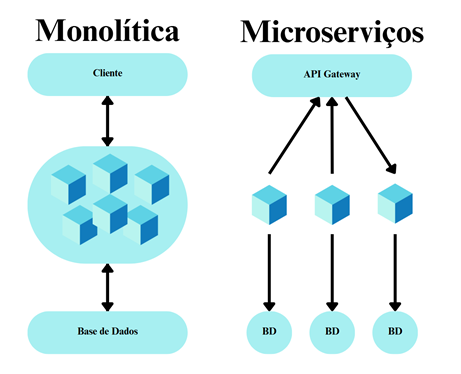
\includegraphics[width=0.6\textwidth]{images/Diagramas/monilitica_vs_microservicos.png}
    \caption{Comparação entre arquitetura monolítica e arquitetura de microsserviços}
    \label{fig:monolitica_microservicos}
\end{figure}

\clearpage

\subsection{De SOA a Microsserviços}


O conceito de decompor aplicações monolíticas em serviços autónomos não é novo. As Arquiteturas Orientadas a Serviços (SOA) surgiram no final dos anos 1990 e início dos anos 2000, como uma primeira forma de abordar os problemas impostos pelas arquiteturas monolíticas. Numa arquitetura deste tipo, as aplicações são organizadas como uma coleção de serviços que interagem por meio de um “barramento” de mensagens - \textit{Enterprise Service Bus} (ESB). Um ESB é um sistema de \textit{middleware} que permite a comunicação entre serviços distintos numa SOA. O ESB atua como um único intermediário central que gere toda a integração, faz o encaminhamento de mensagens, a transformação de dados e aplica as políticas de segurança definidas para os vários serviços do sistema. Embora um ESB simplifique a integração inicial, a sua centralização cria dependências e um potencial ponto de falha do sistema. Fragilidades como estas, fizeram com que se procurassem alternativas mais descentralizadas, como as arquiteturas baseadas em microsserviços \cite{Aziz2020}.

Embora as SOA tenham introduzido avanços significativos na modularização de sistemas, também criaram alguns desafios consideráveis, nomeadamente:


\begin{itemize}
    \item \textbf{Complexidade excessiva.} A utilização de ESB centralizados introduziu um ponto único de falha e complexidade operacional;
    \item \textbf{Rigidez nos contratos de serviços.} A realização de alterações nos serviços do sistema exigiam mudanças pesadas no barramento e nos consumidores.
    \item \textbf{Foco excessivo em tecnologias pesadas.} Padrões como SOAP (Simple Object Access Protocol) e WS-*, um conjunto de especificações de \textit{Web Services} que inclui funcionalidades como segurança, autenticação e transações distribuídas, requeriam a utilização de mensagens estruturadas em XML e contratos rígidos entre serviços. Embora estes protocolos garantissem interoperabilidade padronizada e mecanismos avançados de fiabilidade e segurança, introduziam também uma camada significativa de complexidade, tornando o processo de integração mais pesado, rígido e pouco ágil.

\end{itemize}

A arquitetura de microsserviços pode ser vista como uma evolução pragmática das SOA, mas focada na simplicidade, na independência e na automação de operações. Numa arquitetura de microsserviços, o barramento central é eliminado. Cada serviço comunica diretamente com os outros serviços, o que permite eliminar muitas das complexidades associadas aos tradicionais sistemas orientados a serviços.

A Figura \ref{fig:soa_microservicos} ilustra estas diferenças, evidenciando a centralização do ESB nas arquiteturas SOA em contraste com a comunicação distribuída e independente entre microsserviços.


\begin{figure}[H]
    \centering
    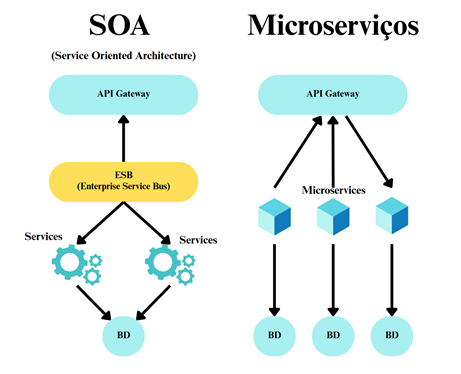
\includegraphics[width=0.6\textwidth]{images/Diagramas/soa_vs_microservicos.png}
    \caption{Comparação entre arquitetura SOA e arquitetura de microsserviços}
    \label{fig:soa_microservicos}
\end{figure}

\subsection{Fatores Tecnológicos e Organizacionais}

O surgimento dos microsserviços não pode ser atribuído apenas a fatores técnicos. Os fatores organizacionais também desempenharam um papel crucial nesse processo. Três dos movimentos principais que impulsionaram esta evolução foram \cite{Newman2015}:

\begin{itemize}
    \item \textbf{Computação em Nuvem.} A elasticidade da nuvem permitiu que aplicações fossem dimensionadas dinamicamente, o que incentivou arquiteturas a tirar partido dessa flexibilidade. Os microsserviços encaixam naturalmente nesse modelo, permitindo escalar apenas os componentes necessários.
    \item \textbf{\textit{DevOps} e \textit{Deployment} Contínuo.} A cultura \textit{DevOps} enfatizou a necessidade de integrar desenvolvimento e operações, automatizar pipelines de entrega contínua e reduzir ciclos de feedback. Os microsserviços permitem ciclos de desenvolvimento independentes para cada serviço, o que os permite alinhar com esses princípios.
    \item \textbf{\textit{Containers} e gestão de \textit{containers} } Tecnologias como \textit{Docker} ou \textit{Kubernetes} simplificaram significativamente a criação, o \textit{deploy} e a gestão de serviços independentes, tornando viável, em larga escala, o modelo dos microsserviços.
\end{itemize}

Segundo \cite{Lewis2014}, a capacidade de alinhar arquitetura de software com estruturas organizacionais ágeis, inspiradas na "Lei de \textit{ Conway}", foi um dos principais catalisadores para a adoção dos microsserviços. A “Lei de \textit{ Conway}”, formulada por Melvin Conway em 1968, estabelece que \textit{ "any organization that designs a system (defined broadly) will produce a design whose structure is a copy of the organization's communication structure"} \cite{Bailey2013} ("qualquer organização que projeta um sistema (em sentido amplo) inevitavelmente produzirá um design cuja estrutura é uma cópia da estrutura de comunicação da organização"). Essa observação implica que as estruturas organizacionais moldam, de maneira direta ou indireta, a arquitetura dos sistemas que desenvolvem.



\subsection{Popularização dos Microsserviços}

O termo microservices começou a ganhar popularidade em conferências técnicas por volta de 2011-2012, sendo posteriormente popularizado pelos trabalhos de autores como James Lewis, Martin Fowler e Sam Newman \cite{Lewis2014,Newman2015}. Empresas pioneiras como Netflix, Amazon, e Uber demonstraram publicamente os benefícios de arquiteturas baseadas em microsserviços, mostrando que era possível construir sistemas resilientes, escaláveis e altamente disponíveis a partir da composição de múltiplos serviços pequenos e independentes.
A experiência e dimensão dessas empresas inspirou uma grande adoção no setor, suportada por uma nova geração de ferramentas de monitorização e gestão distribuída, plataformas de infraestrutura como serviço (IaaS) e metodologias ágeis de desenvolvimento.
Atualmente, os microsserviços são amplamente reconhecidos como uma escolha estratégica para sistemas que exigem alta escalabilidade, independência organizacional e ciclos de entrega rápidos 
\cite{Dragoni2017}. No entanto, essa popularidade não elimina a complexidade técnica e organizacional que a arquitetura de microsserviços impõe, tema que será aprofundado nas próximas secções.


\section{O que são microsserviços?}

Após as limitações evidenciadas pelas arquiteturas monolíticas e a emergência de novos paradigmas tecnológicos e organizacionais, os microsserviços consolidaram-se como uma abordagem inovadora para o desenvolvimento de sistemas distribuídos modernos.

Nesta secção caracteriza-se a arquitetura de microsserviços, destacando as suas principais propriedades no cenário atual de engenharia de software.

\subsection{Definição Formal}

Um microsserviço é uma unidade modular de software criada com o intuito de executar uma funcionalidade especifica integrada num sistema maior. Os microsserviços são independentes e autónomos, podendo assim serem desenvolvidos, testados e escalados separadamente de qualquer outro componente do sistema \cite{Jamshidi2018}. A principal característica dos microsserviços é a separação de responsabilidades. Cada serviço tem o seu propósito no contexto do sistema geral e, por isso, deve executar apenas o seu código, focando-se num único problema, aquilo que realmente lhe compete \cite{Newman2015}. Estes serviços são flexíveis e altamente escaláveis. Além disso permitem a utilização de tecnologias distintas na sua implementação; bem como o desenvolvimento paralelo de serviços e dimensionamento granular por serviço (isto é, a capacidade de escalar apenas os serviços que efetivamente necessitam de mais recursos) \cite{Lewis2014}. Mais do que o tamanho do código, o termo "micro" enfatiza a responsabilidade limitada de cada serviço e a independência operacional, permitindo que estes sejam desenvolvidos, implementados e escalados de maneira isolada. Segundo \cite{Dragoni2017} o conceito de microsserviços surgiu como um refinamento de princípios preexistentes, como modularidade, separação de responsabilidades e princípios do desenvolvimento das SOA, mas com ênfase na autonomia e no alinhamento com domínios de negócio.


\subsection{Princípios e Principais Características}

Podemos caracterizar uma arquitetura de microsserviços como tendo as seguintes características:

\begin{itemize}
    \item \textbf{Autonomia de desenvolvimento e \textit{deployment}.} Cada microsserviço pode ser desenvolvido, testado, implementado e mantido de forma independente \cite{Newman2015}.
    
    \item \textbf{Especialização funcional.} Os serviços são organizados em torno de capacidades de negócio específicas, refletindo o princípio de responsabilidade única \cite{Newman2015}.
    
    \item \textbf{Comunicação leve.} Os microsserviços utilizam protocolos de comunicação simples, como REST sobre HTTP, gRPC ou filas de mensagens assíncronas \cite{Dragoni2017}.
    
    \item \textbf{Independência tecnológica.} Os serviços podem ser implementados em diferentes linguagens de programação ou \textit{frameworks}, promovendo poliglotismo arquitetural 
    \cite{Richardson2018}.
    
    \item \textbf{Escalabilidade granular.} Serviços com maior procura podem ser escalados individualmente, permitindo alocação eficiente de recursos \cite{Lewis2014}.
    
    \item \textbf{Observabilidade.} Cada serviço é projetado para expor métricas, logs e \textit{tracing} distribuído, possibilitando monitorização e diagnóstico isolados \cite{Soldani2018}.
\end{itemize}


Este conjunto de princípios alinha a arquitetura de microsserviços a práticas modernas de desenvolvimento ágil, DevOps e computação em nuvem.

\subsection{Componentes Típicos em Arquiteturas de microsserviços}

Geralmente, a implementação prática de microsserviços envolve diversos componentes arquiteturais adicionais, momeadamente:

\begin{itemize}
    \item \textbf{APIs Públicas.} Cada serviço expõe a sua funcionalidade por meio de uma interface bem definida, normalmente baseada em padrões como RESTful APIs ou gRPC.

    \item \textbf{As Base de Dados são Privadas.} Cada microsserviço é responsável pela sua própria persistência de dados, evitando assim dependências diretas entre serviços \cite{Dragoni2017}.

    \item \textbf{Mensagens Assíncronas.} A comunicação baseada em eventos, utilizando tecnologias como Kafka, RabbitMQ ou SQS, reduz o acoplamento entre serviços e facilita a escalabilidade horizontal.

    \item \textbf{Service Discovery e Load Balancing.} Estes mecanismos automáticos são utilizados para fazerem a localização e o balanceamento de serviços dinâmicos em ambientes distribuídos \cite{Newman2015}.

    \item \textbf{API Gateway.} Uma API que serve para unificar o acesso externo aos serviços e gerir autenticação, encaminhamento, \textit{ caching} e controlo de versões \cite{Richardson2018}.
\end{itemize}


Estes componentes são fundamentais para garantir que uma arquitetura baseada em microsserviços seja robusta, escalável e de fácil manutenção.

\subsection{Comparação com outras Arquiteturas}

Após a apresentação dos princípios e componentes fundamentais da arquitetura de microsserviços, torna-se pertinente posicioná-la relativamente a outras abordagens arquiteturais, como o modelo monolítico e a SOA. Esta comparação é essencial para compreender as diferenças estruturais e organizacionais que motivam a adoção dos microsserviços em determinados contextos. Embora as três abordagens procurem suportar a construção de sistemas robustos e escaláveis, estas diferem significativamente quanto ao seu âmbito funcional, à forma de comunicação entre componentes e à autonomia de desenvolvimento e operação. Enquanto o modelo monolítico centraliza toda a aplicação num único bloco, com forte acoplamento interno, e a SOA tradicional procura modularizar sistemas através de serviços de grande escala coordenados por infraestruturas centrais (como ESBs), a arquitetura de microsserviços distingue-se pela sua granularidade fina, descentralização operacional e leveza na comunicação entre componentes.

Segundo \cite{Newman2015} e \cite{Dragoni2017}, os microsserviços são concebidos para que cada serviço corresponda a uma capacidade de negócio específica, podendo ser desenvolvido, implementado e escalado de forma totalmente autónoma, sem dependências centralizadas.

A Tabela~\ref{tab:comparacao_arq} sintetiza as principais diferenças entre as três abordagens arquiteturais, destacando aspetos como o âmbito funcional, modelo de comunicação, estratégia de \textit{deployment}, gestão de dados e autonomia de desenvolvimento. Esta comparação permite observar de forma clara a evolução de um modelo fortemente centralizado para arquiteturas cada vez mais distribuídas e independentes, evidenciando o papel dos microsserviços enquanto paradigma orientado à escalabilidade organizacional e técnica.

\begin{table}[h]
\centering
\caption{Comparação entre Arquitetura Monolítica, SOA e Microsserviços}
\label{tab:comparacao_arq}
\begin{tabular}{|p{3.3cm}|p{3.3cm}|p{3.3cm}|p{3.3cm}|}
\hline
\textbf{Característica} & \textbf{Arquitetura Monolítica} & \textbf{Arquitetura SOA} & \textbf{Arquitetura de Microserviços} \\ \hline

Âmbito funcional & Abrangente e integrado & Serviços de grande escala & Serviços pequenos e focados \\ \hline

Comunicação & Interna (memória local) & Middleware corporativo (ESB) & APIs leves (HTTP/gRPC) \\ \hline

\textit{Deployment} & Único e centralizado & Parcial, frequentemente acoplado ao ESB & Independente por serviço \\ \hline

Dados & Centralizados & Parcialmente descentralizados & Totalmente descentralizados \\ \hline

Autonomia no desenvolvimento & Reduzida & Moderada & Elevada \\ \hline
\end{tabular}
\end{table}


\section{Os Desafios das Arquiteturas de Microsserviços}

A arquitetura de microsserviços representa uma mudança paradigmática no desenvolvimento de sistemas de software, uma promessa de maior escalabilidade, flexibilidade e capacidade de inovação. Porém, na prática, a construção e a operação de sistemas baseados em microsserviços trazem consigo um conjunto de desafios técnicos e organizacionais que não podem ser ignorados. De seguida, serão analisados os principais aspetos relacionados com a organização de sistemas de microsserviços, bem como os desafios emergentes da sua adoção em larga escala.

\subsection{Organização de Sistemas de Microsserviços}

Os sistemas baseados em microsserviços são compostos por um conjunto de serviços pequenos, especializados e autonomamente desenvolvidos. A sua organização não se limita à existência de vários serviços independentes, mas exige uma conceção cuidadosa das relações entre serviços, das suas formas de comunicação e da delimitação das suas fronteiras \cite{Railic2021,Lewis2014}. 

A comunicação entre microsserviços pode ser síncrona, utilizando APIs RESTful ou gRPC, ou assíncrona, através de sistemas de filas, como \textit{ Apache Kafka} ou \textit{ RabbitMQ}. A comunicação síncrona facilita o desenvolvimento inicial, mas introduz dependências temporais entre serviços, enquanto a comunicação assíncrona promove maior tolerância a falhas, embora acrescente alguma complexidade na gestão da consistência dos dados e na monitorização de transações distribuídas.

A gestão das fronteiras de serviços é um aspeto crucial. Um serviço deve encapsular uma capacidade de negócio bem definida, evitando tanto o excesso de granularidade, que aumenta a complexidade operacional, como a agregação de múltiplas funcionalidades distintas, que reintroduz problemas típicos de arquiteturas monolíticas.

Técnicas como \textit{Domain-Driven Design} (DDD) \cite{Rogers2022} são frequentemente utilizadas para identificar limites de contexto adequados e promover o bom funcionamento interno de cada serviço. A dependência de componentes como \textit{ API Gateways}, mecanismos de \textit{service discovery} e comunicação assíncrona, referidos anteriormente, não deve ser vista apenas como um requisito tecnológico, mas como uma estratégia fundamental para garantir a escalabilidade, resiliência e segurança dos serviços.

\subsection{Principais Desafios Técnicos}

Apesar das vantagens teóricas, a implementação prática de sistemas baseados em microsserviços traz um conjunto significativo de desafios técnicos que se intensificam com o aumento da complexidade e da escala do sistema. A comunicação distribuída é um dos principais pontos de fragilidade: a utilização de redes para interligar serviços introduz atrasos variáveis, falhas de ligação e a necessidade de implementar mecanismos de \textit{retry}, \textit{circuit breaker} e \textit{timeouts} devidamente controlados \cite{Nygard2018,Newman2015}. Além disso, a gestão de APIs torna-se crítica, exigindo práticas rigorosas de versionamento para evitar incompatibilidades em tempo de execução \cite{Richardson2018}.

A gestão de dados distribuídos constitui outro desafio importante. Ao promover a descentralização dos repositórios de dados, a arquitetura de microsserviços inviabiliza a utilização de transações ACID tradicionais entre serviços. Como alternativa, padrões como \textit{Sagas} e a adoção de consistência eventual tornam-se necessários, aumentando a complexidade do desenvolvimento e das operações. A monitorização de sistemas distribuídos exige uma abordagem abrangente de observabilidade: métricas detalhadas por serviço, logs estruturados e \textit{tracing} distribuído são essenciais para a deteção precoce de problemas e para a análise eficaz de incidentes \cite{Burns2015}. Ferramentas como \textit{ Prometheus}, \textit{ Grafana} e \textit{ Jaeger} têm sido amplamente utilizadas para este fim, mas exigem configuração e manutenção especializadas.

A gestão de \textit{deployments} e versões em ambientes de microsserviços também se torna mais complexa. A coordenação de atualizações entre serviços dependentes, a manutenção da compatibilidade de APIs e a implementação de estratégias de \textit{deployment} seguras, como \textit{blue-green deployments} e \textit{canary releases}, são práticas indispensáveis para reduzir o risco de interrupções de serviço \cite{Humble2010}.

\subsection{Principais Desafios Organizacionais}

Para além das dificuldades técnicas, a adoção de microsserviços implica grandes transformações na organização das equipas de desenvolvimento e na cultura empresarial. A autonomia das equipas é um dos princípios fundamentais desta abordagem: cada equipa deve ser responsável pelo ciclo de vida completo dos serviços que desenvolve, desde a conceção até à operação em produção. Esta autonomia reduz a necessidade de coordenação centralizada, mas exige uma forte disciplina na gestão de interfaces e na comunicação entre equipas. A Lei de \textit{ Conway} ensina que a arquitetura dos sistemas tende a refletir a estrutura de comunicação da organização \cite{Bailey2013}. Assim, para beneficiar das vantagens dos microsserviços, é necessário que as fronteiras organizacionais estejam alinhadas com as dos serviços, promovendo equipas pequenas, multifuncionais e responsáveis por domínios de negócio bem delimitados.

A maturidade em práticas de \textit{ DevOps} é outro requisito essencial. A automação de pipelines de integração e entrega contínuas, a gestão centralizada de configurações e a monitorização proativa são práticas indispensáveis para garantir a eficácia operacional em ambientes de microsserviços. Organizações que não possuam essa maturidade tendem a enfrentar dificuldades na gestão da complexidade e na manutenção da fiabilidade dos sistemas \cite{Lewis2014}.

Finalmente, a cultura de responsabilização deve ser reforçada: cada equipa não deve apenas entregar código funcional, mas assumir a responsabilidade contínua pela qualidade, desempenho e estabilidade dos seus serviços em produção. Este paradigma, frequentemente resumido na expressão \textit{"you build it, you run it"}, requer mudanças culturais significativas e um compromisso claro com a excelência operacional \cite{Khan2022}.


\section{Arquiteturas de Microsserviços em Grande Escala}

A implementação de microsserviços em grande escala apresenta desafios únicos em termos de escalabilidade, resiliência e orquestração. Com o aumento da complexidade das aplicações, as soluções tradicionais baseadas em arquiteturas monolíticas não são suficientes para suportar exigências de alta disponibilidade e escalabilidade. Para lidar com sistemas complexos compostos por centenas ou milhares de microsserviços, é fundamental adotar práticas e tecnologias específicas que garantam o bom funcionamento e a escalabilidade das plataformas.

\subsection{Escalabilidade Horizontal}

A escalabilidade horizontal é um dos principais benefícios oferecidos pelos microsserviços, permitindo que os serviços sejam escalados individualmente conforme a demanda. Esta abordagem contrasta com a escalabilidade vertical, comum em sistemas monolíticos, onde a capacidade do sistema é aumentada através do reforço de um único componente \cite{Blinowski2022}. Nos microsserviços, cada serviço pode ser replicado de forma independente para lidar com picos de carga sem impactar outros serviços.

A gestão da escalabilidade horizontal em ambientes distribuídos exige ferramentas de orquestração como o \textit{Kubernetes}, que permitem o dimensionamento automático dos serviços com base em métricas de desempenho em tempo real. O \textit{ Kubernetes} facilita a criação, gestão e monitorização de \textit{containers}, permitindo que os microsserviços sejam escalados automaticamente de acordo com a carga de trabalho \cite{Rocha2023}. Este tipo de escalabilidade garante que os sistemas sejam capazes de lidar com grandes volumes de tráfego sem sobrecarregar recursos ou comprometer a disponibilidade.

\subsection{Gestão do Estado dos Serviços}

Em sistemas distribuídos, a gestão do estado dos serviços é um desafio crítico. No modelo de microsserviços, é comum que cada serviço tenha a sua própria base de dados, promovendo a descentralização do armazenamento. Embora esta abordagem permita maior flexibilidade e agilidade no dimensionamento dos serviços, ela também traz desafios no que diz respeito à consistência dos dados.

A descentralização dos dados pode exigir o uso de técnicas como \textit{event sourcing} e \textit{CQRS} (Command Query Responsibility Segregation), que ajudam a garantir a integridade dos dados entre os serviços \cite{Richardson2018}. Além disso, a sincronização entre serviços independentes pode ser complexa, especialmente quando se lida com falhas de rede e inconsistências temporárias. O uso de comunicação assíncrona e sistemas de filas de mensagens, como \textit{ Kafka} ou \textit{ RabbitMQ}, permite que os microsserviços comuniquem de forma eficiente mesmo em cenários com alta latência ou falhas temporárias \cite{Dragoni2017}.

\subsection{Orquestração e Automação}

A orquestração e automação são fundamentais para a gestão de microsserviços em grande escala. Ferramentas como o Kubernetes não só gerem a criação e escalabilidade dos serviços, mas também garantem mecanismos de \textit{self-healing}, reiniciando ou substituindo automaticamente serviços que falham, minimizando o impacto nos utilizadores finais \cite{Burns2016}. 

Além disso, a automação do processo de \textit{deployment} é um fator crítico. Tecnologias de \textit{CI/CD} (Integração Contínua/Entrega Contínua), combinadas com \textit{ Kubernetes} e \textit{ Docker}, possibilitam o \textit{deployment} contínuo e a validação automática de novas versões dos serviços, garantindo atualizações rápidas e seguras, sem interrupção do funcionamento do sistema \cite{Taherizadeh2020}.

Em suma, a implementação de microsserviços em grande escala exige uma abordagem estratégica que combine escalabilidade horizontal eficiente, gestão robusta de estado e orquestração automatizada. Ferramentas como Kubernetes, Docker e sistemas de mensagens assíncronas desempenham um papel fundamental na gestão e operação destas arquiteturas complexas, garantindo que plataformas baseadas em microsserviços possam atender aos requisitos modernos de alta disponibilidade e resiliência.

\clearpage

\section{Microsserviços e Computação em Nuvem}

A integração de microsserviços com plataformas de computação em nuvem transformou a forma como as empresas desenham e operam os seus sistemas. A nuvem oferece uma infraestrutura elástica que facilita a escalabilidade dinâmica, a gestão simplificada e a alta disponibilidade, características essenciais para ambientes de microsserviços. Esta secção explora a relação entre microsserviços e computação em nuvem, destacando as vantagens, desafios e oportunidades que surgem com o uso de tecnologias de nuvem.

\subsection{Arquitetura \textit{Serverless}}

O paradigma \textit{serverless} representa uma evolução dos microsserviços, na qual a gestão da infraestrutura é totalmente abstraída pelo provedor de nuvem. Numa arquitetura \textit{serverless}, como as oferecidas pelo \textit{ AWS Lambda}, \textit{ Azure Functions} e \textit{ Google Cloud Functions}, as equipas de desenvolvimento podem focar-se apenas na lógica de negócio, sem se preocupar com a gestão de servidores, escalabilidade ou manutenção da infraestrutura subjacente \cite{Dragoni2017}. Embora o \textit{serverless} ofereça grande flexibilidade e escalabilidade automática, também apresenta desafios, especialmente quando se lida com tempos de execução curtos e recursos limitados, que podem afetar a performance em sistemas complexos. Ainda assim, a adoção de microsserviços \textit{serverless} permite reduzir significativamente o custo de operação, dado que os utilizadores pagam apenas pelo tempo de execução dos serviços, tornando-se uma escolha vantajosa para muitas aplicações \cite{Richardson2018}.

\subsection{Custo e Eficiência de Escalabilidade}

A escalabilidade de microsserviços na nuvem também traz implicações em termos de eficiência de custos. A nuvem permite que as empresas escalem os seus serviços de acordo com a procura, evitando a necessidade de provisionar recursos fixos. Com ferramentas como o \textit{Auto Scaling} da \textit{ AWS} e o \textit{ Google Kubernetes Engine (GKE)}, as empresas podem ajustar dinamicamente a capacidade dos seus serviços para se adaptarem a picos de tráfego e garantir uma utilização de recursos otimizada \cite{Dragoni2017}. Esta escalabilidade sob demanda permite uma gestão mais eficiente dos custos operacionais, pois as organizações pagam apenas pelos recursos efetivamente consumidos. Além disso, ao combinar computação em nuvem com a orquestração de microsserviços, as empresas conseguem dimensionar os seus sistemas de maneira eficiente, sem comprometer a performance ou a disponibilidade \cite{Blinowski2022}.

\subsection{Desafios da Computação em Nuvem}

Apesar das inúmeras vantagens, a computação em nuvem apresenta desafios que as organizações precisam de abordar ao implementar microsserviços. A dependência de fornecedor \textit{(*vendor lock-in*)} é um dos principais desafios, pois as organizações podem ficar fortemente dependentes das ferramentas e serviços específicos de um provedor de nuvem. Por exemplo, a portabilidade entre plataformas pode ser limitada, dificultando uma eventual migração para outro fornecedor caso as necessidades da empresa evoluam \cite{Richardson2018}.

Outro desafio importante está relacionado com a segurança e a privacidade dos dados, especialmente quando se lida com informação sensível. Embora os fornecedores de nuvem ofereçam mecanismos robustos de segurança, a responsabilidade de garantir configurações adequadas recai sobre a organização, que deve assegurar a proteção de dados em trânsito e em repouso.
